Un hôtel situé à proximité d'un site touristique dédié à la préhistoire propose deux visites dans les environs, celle d'un musée et celle d'une grotte.

\medskip

Une étude a montré que 70\,\% des clients de l'hôtel visitent le musée. De plus, parmi les clients visitant le musée, 60\,\% visitent la grotte.

Cette étude montre aussi que 6\,\% des clients de l'hôtel ne font aucune visite.

On interroge au hasard un client de l'hôtel et on note :

\begin{itemize}
	\item $M$ l'évènement : \og le client visite le musée \fg{} ;
	\item $G$ l'évènement : \og le client visite la grotte \fg.
\end{itemize}

On note $\overline{M}$ l'évènement contraire de $M$,\: $\overline{G}$ l'évènement contraire de $G$, et pour tout évènement $E$, on note $p(E)$ la probabilité de $E$.

Ainsi, d'après l'énoncé, on a : $p\left(\overline{M} \cap \overline{G}\right) = 0,06$.

\begin{wrapstuff}[r,leftsep=1.5em,rightsep=1em]
	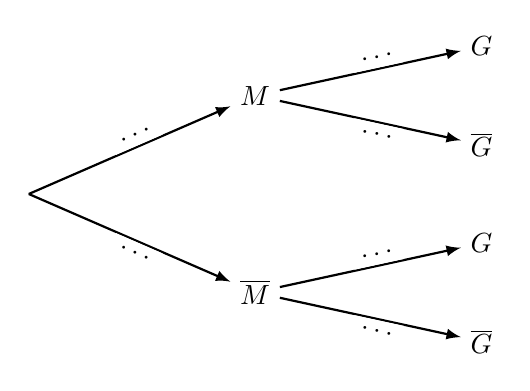
\begin{tikzpicture}[xscale=1,yscale=1]
		\tikzstyle{fleche}=[->,>=latex,thick]
		\tikzstyle{noeud}=[]
		\tikzstyle{etiquette}=[pos=0.55,sloped,fill=white]
		\def\DistanceInterNiveaux{2.5}
		\def\DistanceInterFeuilles{1}
		\def\NiveauA{(0)*\DistanceInterNiveaux}
		\def\NiveauB{(1.15)*\DistanceInterNiveaux}
		\def\NiveauC{(2.3)*\DistanceInterNiveaux}
		\def\InterFeuilles{(-1.25)*\DistanceInterFeuilles}
		\coordinate (R) at ({\NiveauA},{(1.5)*\InterFeuilles}) ;
		\node[noeud] (Ra) at ({\NiveauB},{(0.5)*\InterFeuilles}) {$M$};
		\node[noeud] (Raa) at ({\NiveauC},{(0)*\InterFeuilles}) {$G$};
		\node[noeud] (Rab) at ({\NiveauC},{(1)*\InterFeuilles}) {$\overline{G}$};
		\node[noeud] (Rb) at ({\NiveauB},{(2.5)*\InterFeuilles}) {$\overline{M}$};
		\node[noeud] (Rba) at ({\NiveauC},{(2)*\InterFeuilles}) {$G$};
		\node[noeud] (Rbb) at ({\NiveauC},{(3)*\InterFeuilles}) {$\overline{G}$};
		\draw[fleche] (R)--(Ra) node[etiquette,above] {$\ldots$};
		\draw[fleche] (Ra)--(Raa) node[etiquette,above] {$\ldots$};
		\draw[fleche] (Ra)--(Rab) node[etiquette,below] {$\ldots$};
		\draw[fleche] (R)--(Rb) node[etiquette,below] {$\ldots$};
		\draw[fleche] (Rb)--(Rba) node[etiquette,above] {$\ldots$};
		\draw[fleche] (Rb)--(Rbb) node[etiquette,below] {$\ldots$};
	\end{tikzpicture}
\end{wrapstuff}
%
\begin{enumerate}
	\item 
	\begin{enumerate}
		\item Vérifier que $p_{\overline{M}}\left(\overline{G}\right) = 0,2$, où $p_{\overline{M}}\left(\overline{G}\right)$ désigne la probabilité que le client interrogé
		ne visite pas la grotte sachant qu'il ne visite pas le musée.
		\item L'arbre pondéré ci-contre modélise la situation. Recopier et compléter cet arbre en indiquant sur chaque branche la probabilité associée.
		\item Quelle est la probabilité de l'évènement \og le client visite la grotte et ne visite pas le musée \fg{} ?
		\item Montrer que $p(G) = 0,66$.
	\end{enumerate}
	\item Le responsable de l'hôtel affirme que parmi les clients qui visitent la grotte, plus de la moitié visitent également le musée. Cette affirmation est-elle exacte ?
	\item Les tarifs pour les visites sont les suivants:
	\begin{itemize}
		\item visite du musée : 12 euros;
		\item visite de la grotte : 5 euros.
	\end{itemize}
	On considère la variable aléatoire $T$ qui modélise la somme dépensée par un client de l'hôtel pour ces visites.
	\begin{enumerate}
		\item Donner la loi de probabilité de $T$. On présentera les résultats sous la forme d'un tableau.
		\item Calculer l'espérance mathématique de $T$.
		\item Pour des questions de rentabilité, le responsable de l'hôtel estime que le montant moyen des recettes des visites doit être supérieur à $700$~euros par jour.
		
		Déterminer le nombre moyen de clients par journée permettant d'atteindre cet objectif.
	\end{enumerate}
	\item Pour augmenter les recettes, le responsable souhaite que l'espérance de la variable aléatoire modélisant la somme dépensée par un client de l'hôtel pour ces visites passe à 15 euros, sans modifier le prix de visite du musée qui demeure à $12$ euros. 
	
	Quel prix faut-il fixer pour la visite de la grotte afin d'atteindre cet objectif ? (On admettra que l'augmentation du prix d'entrée de la grotte ne modifie pas la fréquentation des deux sites).
	\item On choisit au hasard $100$ clients de l'hôtel, en assimilant ce choix à un tirage avec remise.
	
	Quelle est la probabilité qu'au moins les trois quarts de ces clients aient visité la grotte à l'occasion de leur séjour à l'hôtel ? 
	
	On donnera une valeur du résultat à $10^{-3}$ près.
\end{enumerate}